% =============================================================================
%  CAB Lab preprint template -- example paper
%  Build:  latexmk -pdf main.tex      (or: make)
%  arXiv:  make arxiv                 (produces arxiv.tar.gz with the .bbl)
% =============================================================================
% Class options: 10pt|11pt|12pt, twocolumn, toc, tocpage, nonatbib, nologo,
%                noheader, draft
\documentclass{cablab}

% ---- Paper-specific packages and macros go here, not in the class ----------
\usepackage{algorithm}
\usepackage{algpseudocode}
\newcommand{\method}{\textsc{GeoNet}\xspace}

% ---- Title block -------------------------------------------------------------
\title{A Concise Title for Your Preprint:\\Optional Subtitle Describing the Contribution}
\shorttitle{A Concise Title for Your Preprint}

\author[1,*]{First Author}
\author[1,*]{Second Author}
\author[2]{Third Author}
\author[1,\dagger]{Christine Allen-Blanchette}

\affiliation[1]{Princeton University}
\affiliation[2]{Another Institution}
\contribution[*]{Equal contribution}
\contribution[\dagger]{Corresponding author}

\begin{abstract}
This is the CAB Lab preprint template. It provides a boxed title panel in translucent Princeton orange with the lab logo, author and affiliation lists, an abstract, keywords and resource links, followed by a single-column body with sans-serif headings, styled captions and a running header. Replace this paragraph with a summary of the problem, the key idea, the evaluation setting and the main result. Keep the abstract to a single paragraph of roughly 150--250 words so that the title panel fits comfortably on the first page together with the opening of the introduction.
\end{abstract}

\keywords{geometric deep learning, equivariance, AI for science, robotics}

\date{\today}
\code{https://github.com/CAB-Lab-Princeton/your-project}
\project{https://cab-lab-princeton.github.io/your-project}
\correspondence{\email{netid@princeton.edu}}

\begin{document}
\maketitle

\section{Introduction}
\label{sec:intro}

Start with the problem and why it matters. Symmetry is one of the most reliable inductive biases in machine learning for the physical sciences: a model whose outputs transform predictably under rotations, translations or permutations needs less data and generalizes further~\cite{bronstein2021geometric,cohen2016group}. \Cref{fig:teaser} shows how a figure, its caption and a cross-reference look in this template.

\begin{figure}[t]
  \centering
  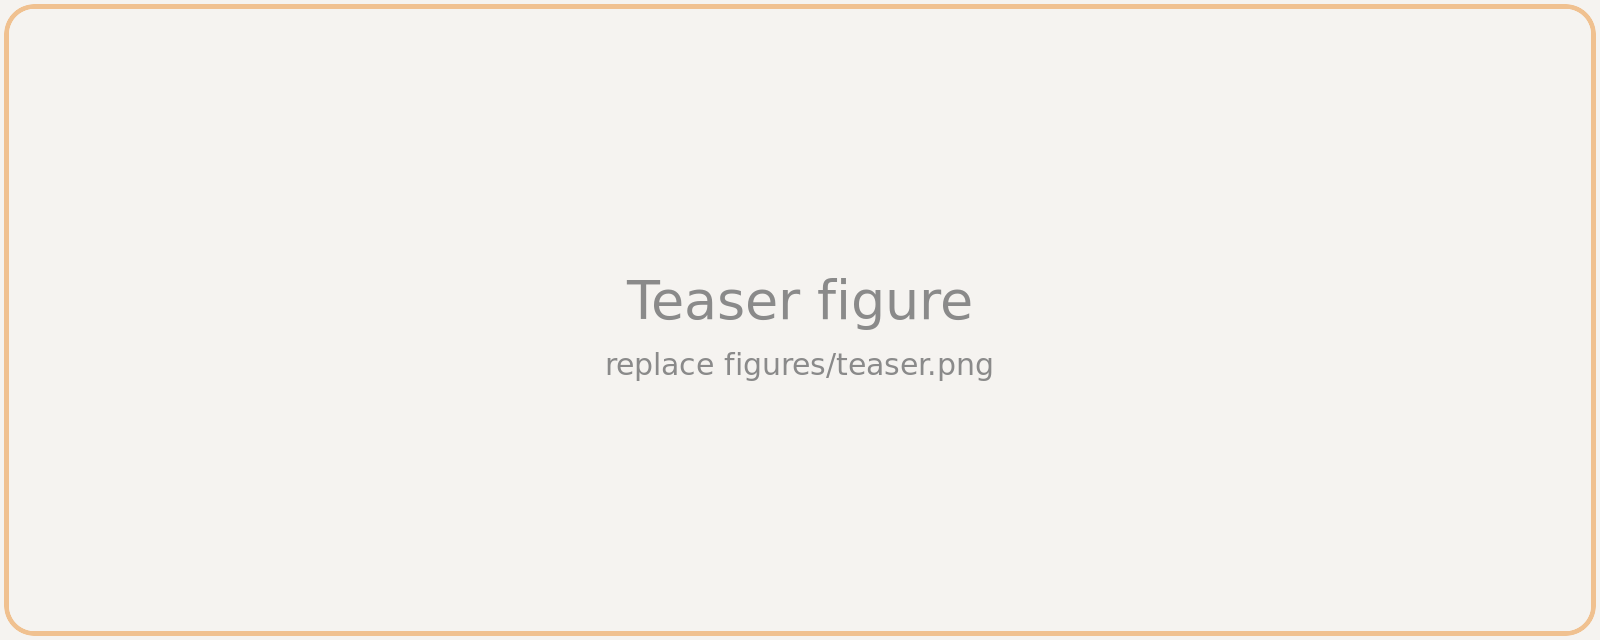
\includegraphics[width=0.82\linewidth]{figures/teaser}
  \caption{\textbf{Teaser figure.} Replace this placeholder with the figure that best summarizes the paper. Captions open with a bold one-line takeaway, then explain what the reader should look at.}
  \label{fig:teaser}
\end{figure}

\parahead{Contributions} State them as a short list.
\begin{itemize}
  \item A new model, \method, that is equivariant by construction (\cref{sec:method}).
  \item A theoretical guarantee on its expressivity (\cref{thm:main}).
  \item Experiments on simulated and real robotic systems (\cref{sec:experiments}).
\end{itemize}

\subsection{Related work}
Group related work by theme in short paragraphs, cite with \verb|\cite|~\cite{vaswani2017attention}, and close with one sentence on how the present work differs.

\section{Method}
\label{sec:method}

Keep paper-specific notation in \texttt{main.tex}. Displayed equations are numbered and can be referenced with \verb|\cref|, as in \cref{eq:equivariance}:
\begin{equation}
  f(\rho_{\mathrm{in}}(g)\,x) = \rho_{\mathrm{out}}(g)\,f(x), \qquad \forall g \in G.
  \label{eq:equivariance}
\end{equation}

\newtheorem{theorem}{Theorem}
\begin{theorem}\label{thm:main}
Every layer of \method commutes with the action of $\mathrm{E}(3)$, hence so does the composed network.
\end{theorem}

\begin{algorithm}[t]
  \caption{Training loop of \method}\label{alg:train}
  \begin{algorithmic}[1]
    \Require dataset $\mathcal{D}$, learning rate $\eta$
    \For{each minibatch $(x, y) \in \mathcal{D}$}
      \State $\hat{y} \gets f_\theta(x)$
      \State $\theta \gets \theta - \eta\,\nabla_\theta \ell(\hat{y}, y)$
    \EndFor
  \end{algorithmic}
\end{algorithm}

\paragraph{Implementation} Run-in paragraph headings use \verb|\paragraph| or \verb|\parahead|. \Cref{alg:train} shows the algorithm environment.

\section{Experiments}
\label{sec:experiments}

Tables use \texttt{booktabs}; the helper \verb|\tablestyle{<colsep>}{<stretch>}| sets compact spacing. Captions of tables sit above the table (\cref{tab:main}).

\begin{table}[t]
  \caption{\textbf{Main results.} Mean $\pm$ std over five seeds; best in bold.}
  \label{tab:main}
  \tablestyle{6pt}{1.15}
  \begin{tabular}{@{}lcccc@{}}
    \toprule
    Method & Equivariant & Params & Error ($\downarrow$) & Time (s) \\
    \midrule
    MLP              & \xmark & 1.2M & $0.412 \pm 0.010$ & 0.8 \\
    Transformer      & \xmark & 3.4M & $0.231 \pm 0.008$ & 2.1 \\
    EGNN             & \cmark & 0.9M & $0.118 \pm 0.004$ & 1.3 \\
    \rowcolor{cabOrange!8}
    \method (ours)   & \cmark & 0.8M & $\mathbf{0.087 \pm 0.003}$ & 1.1 \\
    \bottomrule
  \end{tabular}
\end{table}

Discuss what the numbers show, then add ablations and failure cases.

\section{Conclusion}
Summarize the contribution, state the main limitation honestly, and point to future work.


\section*{Acknowledgments}
Thank the people and funding agencies that supported this work.

\bibliographystyle{unsrtnat}
\bibliography{main}

\beginappendix
\section{Additional details}
\label{app:details}
Appendix sections are lettered automatically after \verb|\beginappendix|.


\end{document}
